\normalfalse \difficilefalse \tdifficiletrue
\correctionfalse

%\UPSTIidClasse{11} % 11 sup, 12 spé
%\newcommand{\UPSTIidClasse}{12}

\exer{Maxpid $\star\star\star$ \label{CIN:01:B2:13:PTSI:18}}
\setcounter{question}{0}\UPSTIcompetence{B2-13}
\index{Compétence B2-13-PTSI}
\index{Maxpid}
\ifcorrection
\else
\marginnote{\textbf{Pas de corrigé pour cet exercice.}}
\fi

\ifprof
\else

Soit le schéma suivant. 
\begin{marginfigure}
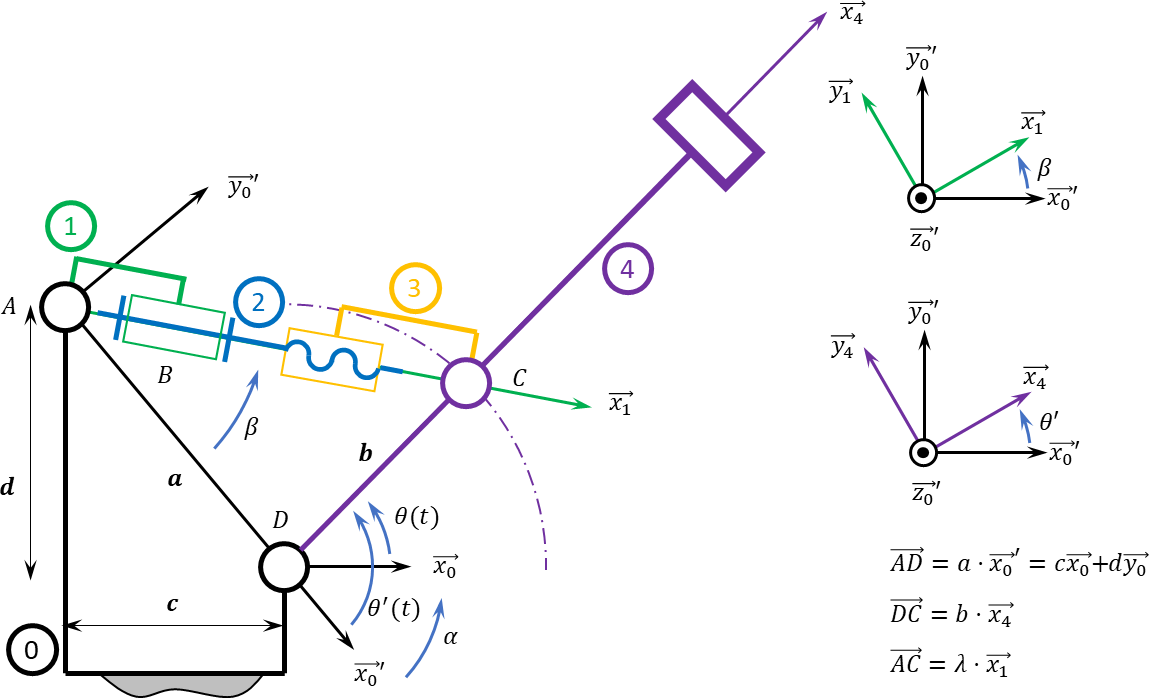
\includegraphics[width=\linewidth]{18_01}
\end{marginfigure}
\fi



\question{Réaliser le paramétrage du mécanisme.}\ifprof
\else
\fi



\ifprof
\else
\marginnote{Corrigé voir \ref{CIN:01:B2:13:PTSI:18}.}

\fi